\documentclass[11pt]{article}

\usepackage{amsmath}
\usepackage{amsfonts}
\usepackage[margin=1in]{geometry}
\usepackage{enumitem}
\usepackage{graphicx}
\usepackage[colorlinks]{hyperref}
\usepackage{longtable}

\usepackage{helvet}
\renewcommand{\familydefault}{\sfdefault}

\setlength{\parindent}{0in}

\def\tightlist{}
\def\toprule{}
\def\bottomrule{}

\begin{document}
{\LARGE Homework 9 (Due November
18th)}\label{homework-9-due-november-18th}

{\Large 1. Modeling the motion of a charged particle in a magnetic
field}\label{modeling-the-motion-of-a-charged-particle-in-a-magnetic-field}

We have shown that the motion of a charged particle in a constant
magnetic is a circular when the initial velocity is perpendicular to the
field. In this problem, you will complete the code in a Jupyter
notebook, which you should
\href{../jupyter/HW9-MotionOfChargeInMagneticField.ipynb}{download} (you
can
\href{https://github.com/dannycab/phy481msu/blob/gh-pages/jupyter/HW9-MotionOfChargeInMagneticField.ipynb}{view
it here}), to model the motion of a proton in a magnetic field.

\begin{enumerate}
\def\labelenumi{\arabic{enumi}.}
\tightlist
\item
  You first task is to read through the code and complete the
  integration loop to compute the trajectory of the proton and plot it
  in 3D. (You might need to look up how to construct a 3D plot.) For
  this first case, you should expect a simple circular orbit because the
  proton starts it's motion moving perpendicular to the magnetic field.
\item
  Once you have your code working for part 1, change it to give the
  proton a component of velocity along the direction of the magnetic
  field. What does the resulting motion look like? Explain qualitatively
  why it should look like that.
\item
  Now add an antiproton to your code and model it's motion along side
  the proton (assume the charges don't interact with each other). How
  does the motion of the antiproton compare to the proton? Explain
  qualitatively why it should look like that.
\end{enumerate}

{\Large 2. Current Density Practice}\label{current-density-practice}

Let's practice writing down some current densities:

\begin{enumerate}
\def\labelenumi{\arabic{enumi}.}
\tightlist
\item
  A sphere (radius \(R\), total charge \(Q\) uniformly distributed
  throughout the volume) is spinning at angular velocity
  \(\omega \hat{z}\) about its center, which is at the origin. What is
  the volume current density \(\mathbf{J}(r, \theta, \phi)\) at any
  point \((r, \theta, \phi)\) in the sphere? (Don't forget direction
  too!)
\item
  A very thin plastic ring (radius \(R\)) has a constant linear charge
  density, and total charge \(Q\). The ring spins at angular velocity
  \(\omega\) about its center, which is the origin. What is the current
  \(I\), in terms of given quantities? What is the volume current
  density \(\mathbf{J}\) in cylindrical coordinates? (This may be a
  little tricky, since the ring is ``very thin'', there will be some
  \(\delta\) functions. \emph{Hint: write down a formula for
  \(\rho(r,\theta,z)\) first. And, remember that \(\mathbf{J}\) should
  be a vector!)}
\end{enumerate}

{\Large 3. Magnetic field of distributed
currents}\label{magnetic-field-of-distributed-currents}

\begin{figure}[htbp]
\centering
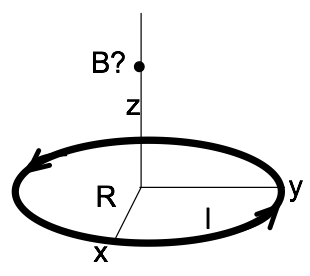
\includegraphics[width=0.3\linewidth]{./images/hw9/ring.png}
\end{figure}

\begin{enumerate}
\def\labelenumi{\arabic{enumi}.}
\tightlist
\item
  Compute the magnetic field \(\mathbf{B}(0,0,z)\) along the \(z\)-axis
  for a current loop (current \(I\), radius \(R\), sitting in \(x-y\)
  plane, centered around the \(z\)-axis). It is shown in the figure
  above.
\item
  Last week we had a DVD (radius \(R\)) with a fixed, constant, uniform
  surface electric charge density \(\sigma\) everywhere on its top
  surface (figure below). It was spinning at angular velocity \(\omega\)
  about its center (the origin). You found the current density
  \(\mathbf{K}\) at a distance \(r\) from the center. Use that result to
  find the magnetic field \(\mathbf{B}(0,0,z)\) at any distance \(z\)
  directly above the origin. (Part 1 above might help.)
\item
  Does your answer to part 2 seem reasonable? Please check it, with
  units, and some limiting behaviors (e.g.~what do you expect if
  \(R \rightarrow 0\)? \(\omega \rightarrow 0\)?
  \(z\rightarrow \infty\)? For this last one, don't just say ``it goes
  to zero. This is a dipole, so \(B\) should go to 0 like \(1/z^3\).
  (Right?) Show that it does!
\end{enumerate}

\begin{figure}[htbp]
\centering
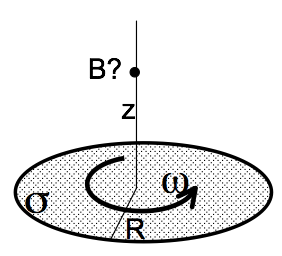
\includegraphics[width=0.3\linewidth]{./images/hw9/disk.png}
\end{figure}

{\Large 4. Magnetic field of a bent
wire}\label{magnetic-field-of-a-bent-wire}

An infinitely long wire has been bent into a right angle turn, as shown.
The ``curvy part'' where it bends is a perfect quarter circle, radius
\(R\). Point P is exactly at the center of that quarter circle. A steady
current \(I\) flows through this wire.

\begin{enumerate}
\def\labelenumi{\arabic{enumi}.}
\tightlist
\item
  Find \(\mathbf{B}\) at point P (magnitude and direction) (\emph{No
  need to derive any formulas ``from scratch'' if you can get them from
  Griffiths' examples!})
\end{enumerate}

\begin{figure}[htbp]
\centering
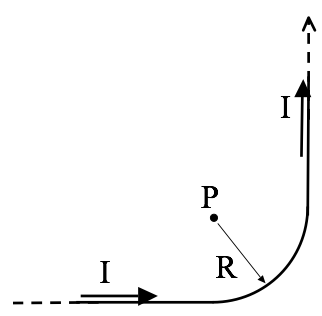
\includegraphics[width=0.3\linewidth]{./images/hw9/bent_wire.png}
\end{figure}

{\Large 5. Estimating the magnetic field of a square
loop}\label{estimating-the-magnetic-field-of-a-square-loop}

\begin{enumerate}
\def\labelenumi{\arabic{enumi}.}
\tightlist
\item
  Find \(\mathbf{B}\) at the exact center of a square current loop
  (current \(I\) running around a wire bent in the shape of a square of
  side \(a\)) (\emph{No need to derive any formulas ``from scratch'' if
  you can get them from Griffiths' examples!})
\item
  If we had such a loop in the lab and wanted \(\mathbf{B}\) at the
  center, we might do the above calculation, but if we were planning an
  experiment and just wanted a rough estimate of the magnetic field, we
  might ``assume a spherical cow'': assume the square was really a
  circle. We've done that problem (\(\mathbf{B}\) at the center of a
  circular loop). It's much simpler than the square! You don't have to
  rederive it, but think back to how we got that result, and why it
  turned out to be a relatively easy application of Biot-Savart. But
  what radius circle would you use, to estimate \(\mathbf{B}\)? You
  might consider finding \(\mathbf{B}\) for the ``inscribed'' and
  ``circumscribed'' circles and then average. How good an approximation
  does that turn out to be? (Can you think of a better way?)
\end{enumerate}

\begin{figure}[htbp]
\centering
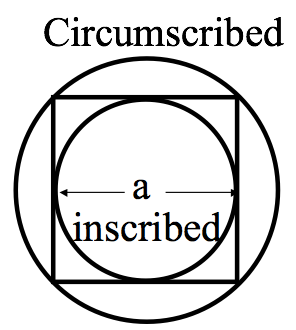
\includegraphics[width=0.3\linewidth]{./images/hw9/square_wire.png}
\end{figure}

{\Large 6. Ampere's Law - themes and
variations}\label{amperes-law---themes-and-variations}

Consider a thin sheet with uniform surface current density.

\begin{figure}[htbp]
\centering
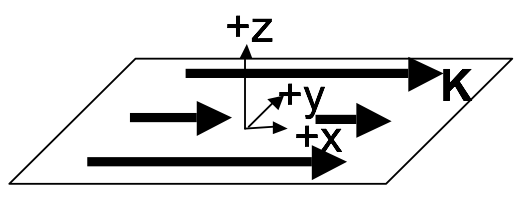
\includegraphics[width=0.5\linewidth]{./images/hw9/sheet_current.png}
\end{figure}

\begin{enumerate}
\def\labelenumi{\arabic{enumi}.}
\tightlist
\item
  Use the Biot-Savart law to find \(\mathbf{B}(x,y,z)\) both above and
  below the sheet, by integration. Note: The integral is slightly nasty.
  Before you turn to WolframAlpha - simplify as much as possible! Set up
  the integral, be explicit about what curly \(R\) is, what \(da'\) is,
  etc, what your integration limits are, etc. Then, make clear
  mathematical and/or physical arguments based on symmetry to convince
  yourself of the direction of the B field (both above and below the
  sheet), and to argue how \(\mathbf{B}(x,y,z)\) depends (or doesn't) on
  \(x\) and \(y\). (If you know it doesn't depend on x or y, you could
  e.g.~choose x=y=0 to simplify\ldots{} But first you must convince us
  that's legit!)
\item
  Now solve the above problem using Ampere's law. (Much easier than part
  1, isn't it?) Please be explicit about what Amperian loop(s) you are
  drawing and why. What assumptions (or results from part 1) are you
  making/using? (\emph{Griffiths solves this problem, so don't just copy
  him, work it out for yourself!})
\item
  Now let's add a second parallel sheet at \(z=+a\) with a current
  running the other way. (Formally, this means
  \(\mathbf{J}=-K_0\delta(z-a)\hat{x}\). Do you understand this
  notation?) Use the superposition principle (do NOT start from scratch
  or use Ampere's law again, this part should be relatively quick) to
  find B between the two sheets, and also \emph{outside} (above or
  below) both sheets. \emph{Does this remind you of a familiar
  electrostatics problem at all? How?}
\item
  Griffiths derives a formula for the B field from a solenoid (Example
  5.9) Rewrite his answer (which is in terms of I) so it is expressed in
  terms of K (See his Fig 5.34 and 5.35 for help with this). Briefly
  compare with part 3, do you see any rough connections?
\end{enumerate}
\end{document}
